\usetikzlibrary{arrows.meta,calc,shapes}
\providecommand{\computer}{%
    
\includegraphics[width=1cm]{../common/Noun_project_216.pdf}
}
\providecommand{\switch}{%
    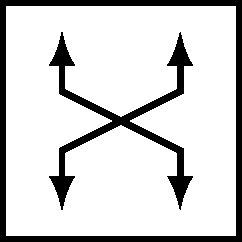
\includegraphics[width=0.9cm]{../common/fig-switch.pdf}
}
\providecommand{\router}{%
    
\includegraphics[width=0.9cm]{../common/fig-router.pdf}
}

\begin{frame}{recall: multi-access media}
\begin{tikzpicture}
\tikzset{
    connect/.style={draw,very thick,arrows={Latex-Circle[width=0.3cm,length=0.3cm]},
        alt=<2>{arrows={Latex-Circle[width=0.3cm,length=0.3cm,red]}}},
    computer/.style={inner sep=0mm,outer sep=0mm,execute at begin node={\computer}},
}
\draw[line width=1mm] (-5,-1.5) coordinate (wire start) -- (5, 1.5) coordinate (wire end);
\foreach \x/\d in {0/5cm,45/4cm,90/3cm,135/4cm,180/5cm,225/4cm,270/3cm,315/4cm} {
    \node[computer] (c-\x) at (\x:\d) {};
    \coordinate (connect-\x) at ($(wire start)!(c-\x.center)!(wire end)$);
    \draw[connect] (c-\x) -- (connect-\x) -- ([turn]0:.1cm);
}
\begin{visibleenv}<2-3>
\node[anchor=north west,fill=white,draw=black,thick,label={[font=\tiny]south:Ali at gwc.org.uk / Alistair1978 via Wikimedia commons / CC-BY-SA 2.5}] 
    (thicknet) at (4, 3.5) {
    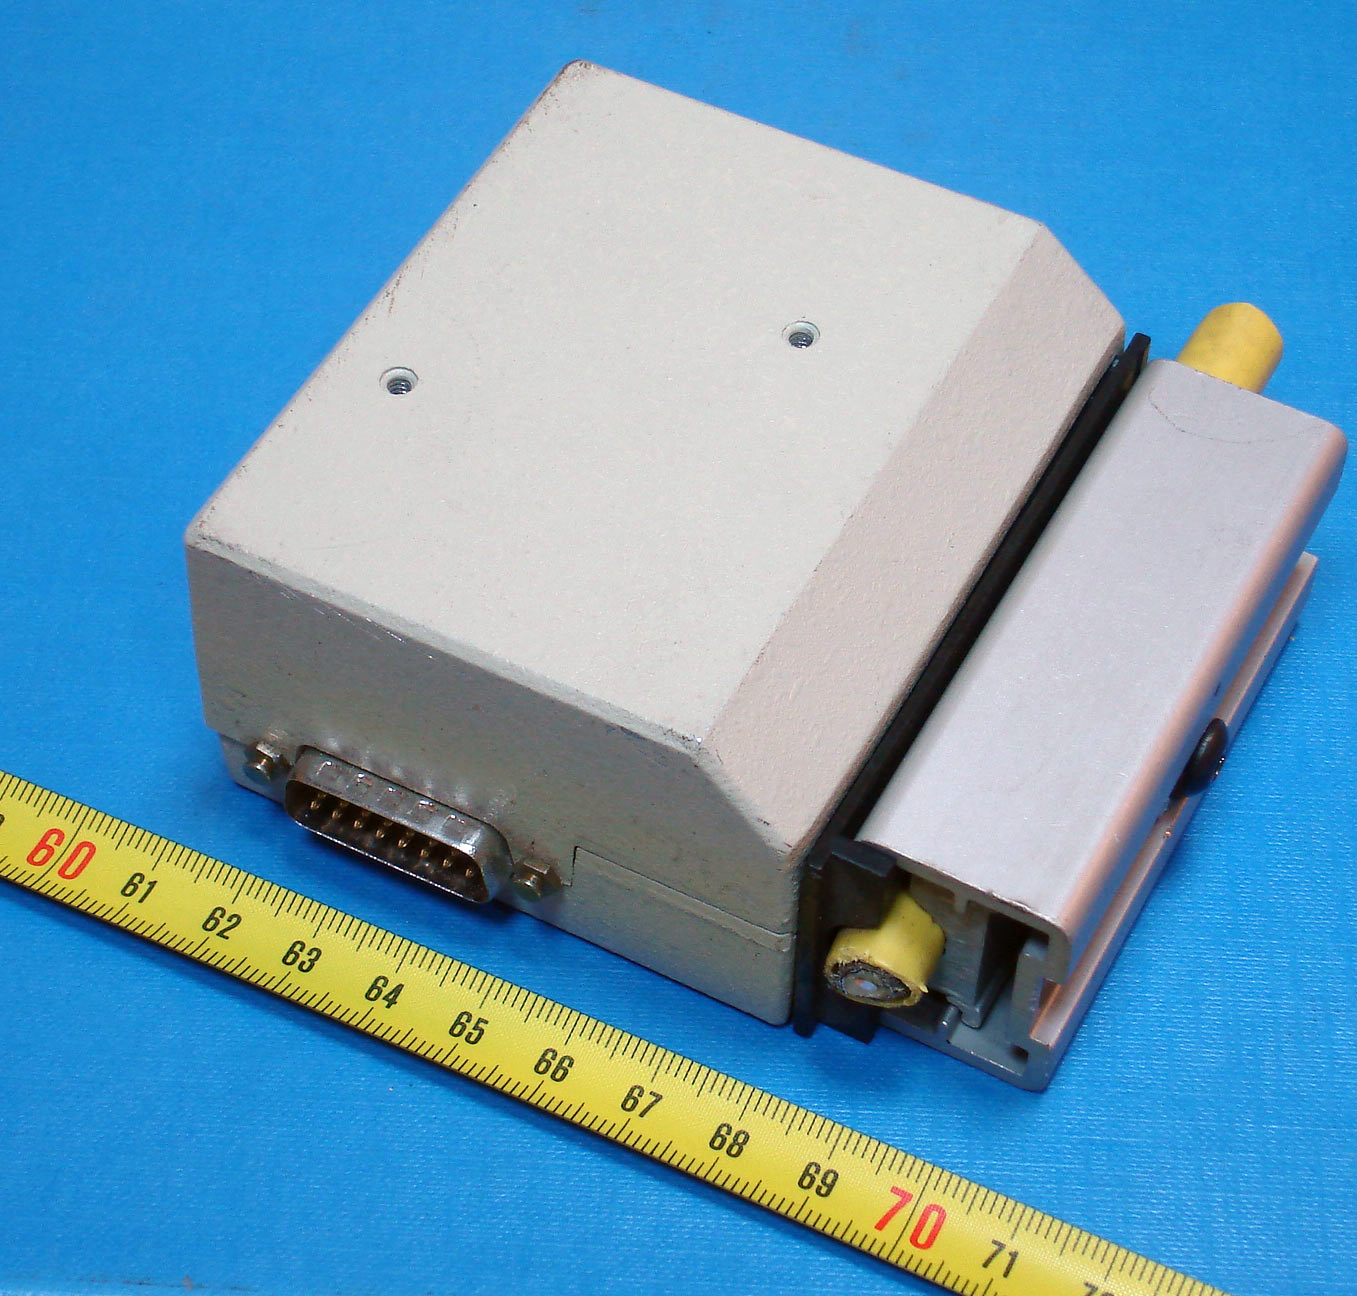
\includegraphics[width=4cm]{../intro/ThicknetTransceiver.jpeg}
};
\end{visibleenv}
\begin{visibleenv}<3>
\node[fill=white,draw=black,thick,anchor=north west] at ([yshift=-0.75cm]thicknet.south west) {
    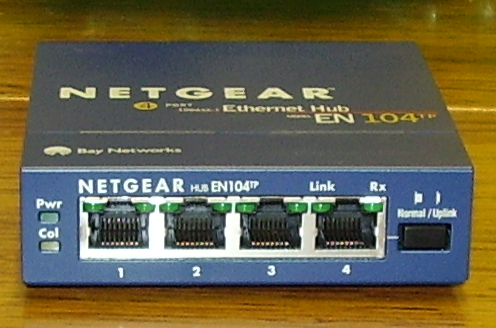
\includegraphics[width=4cm]{../intro/4_port_netgear_ethernet_hub}
};
% FIXME: also fiber splitter
\end{visibleenv}
\end{tikzpicture}
\end{frame}

\begin{frame}{recall: switched network}
\begin{tikzpicture}
\tikzset{
    computer/.style={inner sep=0mm,outer sep=0mm,execute at begin node={\computer}},
    switch/.style={inner sep=0mm,outer sep=0mm,execute at begin node={\switch},
                   alt=<1>{
                       fill=red!10,
                        label={[font=\small,label distance=0mm,text=red]south:`switch'}
                   }},
    connect/.style={draw,very thick,Latex-Latex,alt=<4>{red}},
    connect big/.style={draw,ultra thick,Latex-Latex,alt=<4>{red}},
}
\node[
      cloud,draw,opacity=0.25,very thick,aspect=2,
      minimum width=7cm,minimum height=4cm,
     ] (net-cloud) at (0,0) {};
\foreach \x/\d in {0/5cm,45/4cm,90/3cm,135/4cm,180/5cm,225/4cm,270/3cm,315/4cm} {
    \node[computer] (c-\x) at (\x:\d) {};
}
\node[switch] (s1) at (2,-0.5) {};
\node[switch] (s2) at (-1,0.5) {};
\node[switch] (s3) at (0,-1) {};
\draw[connect] (c-0) -- (s1);
\draw[connect] (c-45) -- (s1);
\draw[connect] (c-315) -- (s1);
\draw[connect] (c-90) -- (s2);
\draw[connect] (c-135) -- (s2);
\draw[connect] (c-180) -- (s2);
\draw[connect] (c-225) -- (s3);
\draw[connect] (c-270) -- (s3);
\draw[connect big] (s1) -- (s2);
\draw[connect big] (s1) -- (s3);
\coordinate (box loc) at (4cm, 4.5cm);
\end{tikzpicture}
\end{frame}

\begin{frame}{hubs and switches}
\begin{tikzpicture}
\node[fill=white,draw=black,thick,label={north:Hub}] (hub) {
    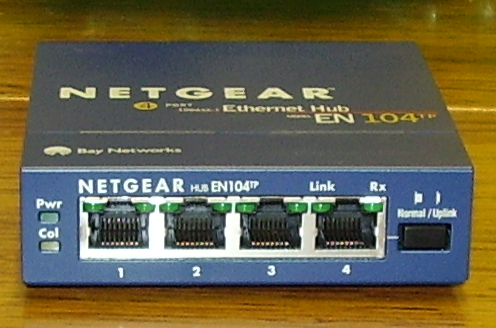
\includegraphics[width=6cm]{../intro/4_port_netgear_ethernet_hub}
};
\node[fill=white,draw=black,thick,anchor=north east,label={north:Switch}] (switch)  at (hub.north west){
    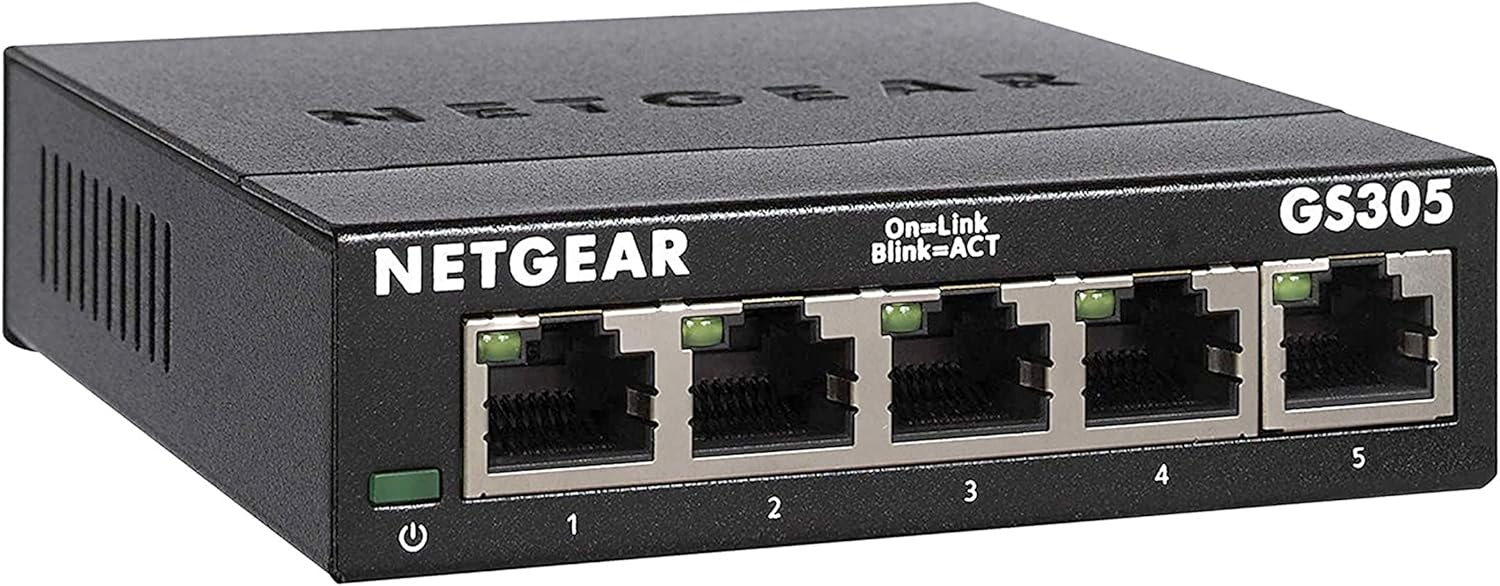
\includegraphics[width=6cm]{../switches/ModernNetgearSwitch}
};
\end{tikzpicture}
\begin{itemize}
\item difference is hidden inside
\item hub: electrically connects hosts --- as if shared wires
\item switch: decides what to send on each output
\end{itemize}
\end{frame}

\begin{frame}{history: multi-access to switched}
    \begin{itemize}
    \item a lot of early networking technology was multi-access
    \item wireless (wifi, cellular) and most home broadband still is
    \vspace{.5cm}
    \item most wired networks are \textit{switched}
        \begin{itemize}
        \item frames mostly directed to correct machine
        \end{itemize}
    \end{itemize}
\end{frame}

\begin{frame}{switching versus routing}
    \begin{itemize}
    \item switches --- forward frames for common network
    \item routers --- forward packets between networks
    \vspace{.5cm}
    \item basically same functionality
    \item differences:
        \begin{itemize}
        \item extra layer for internetwork packets
        \item different mechanism to decide where to forward
        \item switch forwarding typically simpler
        \end{itemize}
    \item will start with simpler switching
    \end{itemize}
\end{frame}

